\documentclass[11pt, a4paper]{article} %or article has only section and below, book and report also have chapter: http://texblog.org/2007/07/09/documentclassbook-report-article-or-letter/

\usepackage[utf8]{inputenc}  % use utf8 encoding of symbols such as umlaute for maximal compatibility across platforms

\usepackage{caption}    		% provides commands for handling caption sizes etc.
%\usepackage[a4paper, left=25mm, right=20mm, top=25mm, bottom=20mm]{geometry}		 % to easily change margin widths: https://www.sharelatex.com/learn/Page_size_and_margins

\usepackage{etoolbox}    % for conditional evaluations!
%\usepackage{fancyverb}   % for syntax highlighting of R code, together with the listings package
\usepackage[bottom]{footmisc}  % I love footnotes! And they should be down at the bottom of the page!
\usepackage{graphicx}        % when using figures and alike
\usepackage[hidelinks]{hyperref}		% for hyperreferences (links within the document: references, figures, tables, citations)
%\usepackage{listings}
\usepackage{lscape}
\usepackage{euler}     % a math font, only for equations and alike; call BEFORE changing the main font; alternatives: mathptmx, fourier, 
%\usepackage{gentium} % for a different font; you can also try: cantarell, charter, libertine, gentium, bera, ... http://tex.stackexchange.com/questions/59403/what-font-packages-are-installed-in-tex-live
\usepackage[margin=1in]{geometry}

%------------------------------------------------------------------------------------------------------
%------- text size settings --------------
%\setlength{\textwidth}{16cm}% 
%\setlength{\textheight}{25cm} %23 
%(these values were used to fill the page more fully and thus reduce the number of pages!)
%\setlength{\topmargin}{-1.5cm} %0
%\setlength{\footskip}{1cm} %
%\setlength{\hoffset}{0cm} %
%\setlength{\oddsidemargin}{1cm}%
%\setlength{\evensidemargin}{-.5cm}%
%\setlength{\parskip}{0cm} % Abstand zwischen Absätzen
% ----------------------------------------------------------------
%\renewcommand{\textfraction}{0.1} % allows more space to graphics in float
%\renewcommand{\topfraction}{0.85}
%\renewcommand{\bottomfraction}{0.65}
%\renewcommand{\floatpagefraction}{0.70}


\frenchspacing %http://texwelt.de/wissen/fragen/1154/was-ist-french-spacing-was-macht-frenchspacing
%------------------------------------------------------------------------------------------------------
%------------------------------------------------------------------------------------------------------

\usepackage{Sweave}
\begin{document}
%%%%%%%%%%%%% this bit is new to Sweave: %%%%%%%%%%%%%%%%%%%%%  
\Sconcordance{concordance:sweave_document_TB.tex:sweave_document_TB.Rnw:%
<<<<<<< Updated upstream
1 39 1 1 0 22 1 1 8 4 1 1 7 1 2 9 1 2 2 4 1 1 4 1 1 1 4 20 1}
=======
1 39 1 1 0 24 1 1 7 1 2 6 1 1 4 1 2 3 1}
>>>>>>> Stashed changes



\title{Appendix}

\author{Torfinn and Carolina}

\maketitle

%------------------------------------------------------------------------------------------------------
%------------------------------------------------------------------------------------------------------


\section{Introduction}%------------------------------------------------------------------------------------------------------

We created an appendix of meta-analysis paper. To be able to visualize the output, we used an example dataset taken from Gibson et al. 2011.

%The dataset to be working with should be named ``data.sub''. The conducted analysis using the function rma from the metafor pacakge should be renamed as such: rma of a random effects model should be named ``rma.RE'' and an rma of a fixed effects model should be named ``rma.FE'' in order for the automatisation to work. IF a meta-regression has been conducted, it should be called ``rma.RE.meta'' or ``rma.FE.meta'' respectively. Other than that, the metafor package in R needs to be installed.  





\begin{figure}
\captionsetup{width=0.6\textwidth}
\centering
\includegraphics[width=1\textwidth]{sweave_document_TB-forest}
\caption{Forest plot of a random effects model. The column on the left represents the study. The weighted percentage is shown as well as the effect size (ES) [+- 95\% CI]}
\label{fig:forestplot}
\end{figure}



%Table with values for ES, SE (ES),pES, CI, I2, Egger value and fasil-sage number. If various rma analysis are run, they can be loaded into this table as well. 
?? How can a an automised table be created for rows from e.g. different rma objects? In our case, we just have one rma object so one row is produced. If the people conduct different rmas for different data subsets, it would be nice to have this in the same table as well!\\
\bigskip




% latex table generated in R 3.1.1 by xtable 1.7-4 package
% Tue Nov 25 09:54:13 2014
\begin{table}[ht]
\centering
\caption{Results of the meta-analysis.ES = Effect Size, Q = Test for residual heterogeneity, $I^2$ = residual heterogeneity, Egger's test and the fails-safe number for publication bias testing.} 
{\footnotesize
\scalebox{0.9}{
\begin{tabular}{rccccccccccc}
  \hline
 & {ES} & \parbox{1cm}{SE of ES} & CI (lb) & CI (ub) & P(ES) & Q & P(Q) & I^2 & Egger & P(Egger) & FSN \\ 
  \hline
Meta-Analysis & -0.28 & 0.12 & -0.52 & -0.04 & 0.02 & 47.05 & 0.12 & 27.22 & -0.44 & 0.66 & 77.00 \\ 
   \hline
\end{tabular}
}
}
\end{table}

\bigskip

%Table of the meta-regression. In this case only for one moderator. 


% latex table generated in R 3.1.1 by xtable 1.7-4 package
% Tue Nov 25 09:54:13 2014
\begin{table}[ht]
\centering
\caption{Results of the meta-regression (mixed-effects model). The model results are shown taking a moderator into account and displaying the coefficients. Results for the whole model are displayed as Q = Test for residual heterogeneity, $I^2$ = residual heterogeneity and QM = Test of Moderators.} 
{\footnotesize
\scalebox{0.9}{
\begin{tabular}{rccccc|ccccc}
  \hline
 & {ES} & \parbox{1cm}{SE of ES} & CI (lb) & CI (ub) & P(ES) & Q & P(Q) & I^2 & QM & P(QM) \\ 
  \hline
Intercept (Africa) & 0.14 & 0.32 & -0.48 & 0.76 & 0.66 & 40.60 & 0.20 & 21.75 & 2.69 & 0.44 \\ 
  Asia & -0.39 & 0.39 & -1.16 & 0.38 & 0.32 &  &  &  &  &  \\ 
  Central America & -0.39 & 0.43 & -1.24 & 0.47 & 0.37 &  &  &  &  &  \\ 
  South America & -0.59 & 0.36 & -1.29 & 0.12 & 0.10 &  &  &  &  &  \\ 
   \hline
\end{tabular}
}
}
\end{table}




To do:

\begin{Schunk}
\begin{Soutput}
[1]  7 11 12 15 21 35
\end{Soutput}
\end{Schunk}

% latex table generated in R 3.1.1 by xtable 1.7-4 package
% Tue Nov 25 09:54:13 2014
\begin{table}[ht]
\centering
\caption{Results of the meta-analysis.ES = Effect Size, Q = Test for residual heterogeneity, $I^2$ = residual heterogeneity, Egger's test and the fails-safe number for publication bias testing.} 
{\footnotesize
\scalebox{0.9}{
\begin{tabular}{rccccccccccc}
  \hline
 & {ES} & \parbox{1cm}{SE of ES} & CI (lb) & CI (ub) & P(ES) & Q & P(Q) & I^2 & Egger & P(Egger) & FSN \\ 
  \hline
Meta-Analysis & -0.28 & 0.12 & -0.52 & -0.04 & 0.02 & 47.05 & 0.12 & 27.22 & -0.44 & 0.66 & 77.00 \\ 
   \hline
\end{tabular}
}
}
\end{table}
A table for the sensitivity analysis. \\

Notes:

Are we going to make two scripts? One for meta and one for metafor or are we going to do a combination? 
Till now it would only work with one rma.RE object with one row and not many. Is is possible to combine specific single values of various rma objects? Can we do this?



To assess possible publication bias, funnel plots can be used for visualization purposes.


\begin{figure}
\captionsetup{width=0.6\textwidth}
\centering
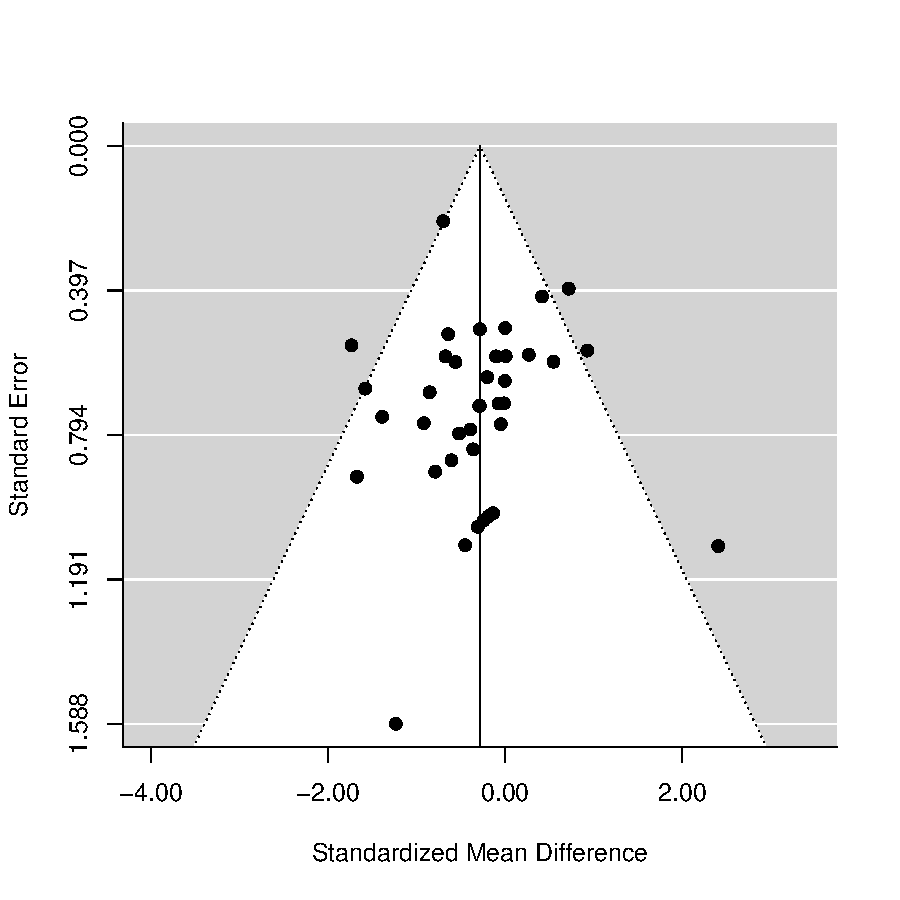
\includegraphics[width=0.7\textwidth]{sweave_document_TB-funnelplot}
\caption{Funnel plot of random effects model displaying possible publication bias. The true ES is displayed by the solid verical line.}
\end{figure}



\begin{figure}
\captionsetup{width=0.6\textwidth}
\centering
\includegraphics[width=1\textwidth]{sweave_document_TB-diagnostics}
\caption{Diagnostic plots for diagnostics of meta analysis. Standardized residual plot, normal Q-Q plot, Baujat heterogeneity plot and Galbrath's radial plot are shown.}
\label{fig:diagnostics}
\end{figure}


\begin{figure}
\captionsetup{width=0.6\textwidth}
\centering
\includegraphics[width=1\textwidth]{sweave_document_TB-forestreg}
\caption{Forest plot of a random effects regression model. The column on the left represents the study. The weighted percentage is shown as well as the effect size (ES) [+- 95\% CI]}
\label{fig:forestplotreg}
\end{figure}

\end{document}
